\chapter{Buying Power: Contracts, Price Arbitrage, and the Strike Price}
\chaptermark{Buying Power}
\label{ch:buying}

Chapter~5 built a machine that flinches away from expensive electricity in minutes. This chapter asks the question that the machine cannot answer for itself: expensive compared to what? The answer is written in a contract. Two mining sites in the same county, drawing the same megawatts through the same weather, can end the year with wildly different power bills because one signed a fixed price in 2021 and the other buys every fifteen minutes at whatever the market says. Before the book can price flexibility, it has to price the electricity, and electricity is not bought at ``the market price.'' It is bought through one of a small menu of contract shapes, and the shape decides what you pay on an average day, what you pay in a crisis, and whether your off switch is connected to anything at all.

\section{The Contract Menu}

Every power contract is an answer to one question: who carries the price risk. At one end of the menu sits the \glossaryterm{power-purchase-agreement}{power purchase agreement} (PPA), a bilateral contract that fixes the volume, price and term of the power bought; the supplier carries the market risk, and charges for the service. At the other end sits the \glossaryterm{index-contract}{index contract}, where the buyer pays the market's settlement price for every interval it consumes; the buyer carries everything. In between sit \glossaryterm{block}{blocks}: fixed prices for fixed slices of the week, hedging some hours and leaving the rest exposed.

These contracts are all on the books of publicly traded Bitcoin miners in Texas, disclosed in enough detail to study because United States securities law makes large companies file their material contracts.

Riot Platforms runs its Rockdale facility, one of the largest Bitcoin mines in the world, on the fixed end of the menu: 345~MW of long-term fixed-price power, contracted in three tranches between May 2020 and November 2022, at fixed prices running to April 2030 for the first two tranches and October 2027 for the third \autocite{riot10k2024}. % src: riot10k2024, Note 20 (130 MW May 2020 + 65 MW Mar 2022 to Apr 2030; 150 MW Nov 2022 to Oct 2027)
The same contract contains the clause this whole book turns on: Riot may elect \emph{not} to consume its fixed-price power and instead sell it back, taking credits against future power bills whenever the spot price makes that the better trade. % src: riot10k2024, Note 20 sell-back election
Hold that clause; Section~\ref{sec:arbitrage} is about what it is worth.

Cipher Mining's Odessa facility sits nearby on the menu: a PPA with Luminant at approximately 2.7 cents per kilowatt-hour, which is \$27/MWh in this book's units, running to at least July 2027 \autocite{cipher10k2024}. % src: cipher10k2024, Luminant Power Agreement ("approximately 2.7 c/kWh")
It is a \glossaryterm{take-or-pay}{take-or-pay} contract: Cipher must accept and pay for at least 66.7~percent of the site's 207~MW capacity every year whether it consumes the power or not. % src: cipher10k2024 (66.7% of 207 MW, take-or-pay)
Like Riot, Cipher can route unneeded power back to the market through its supplier; those power sales brought in \$5.4~million in 2024 and \$9.9~million in 2023. % src: cipher10k2024, power sales proceeds
Cipher's other Texas sites, Bear and Chief, have no fixed-price contract at all: they buy at the spot price and manage cost purely by pausing when prices are high. % src: cipher10k2024 ("do not currently have fixed price power purchase agreements"; curtailment software)

IREN went furthest toward the bare end. In August 2024 it paid \$7.2~million to close out its remaining hedges and moved its Childress site to buying directly from the ERCOT wholesale spot market \autocite{iren10k2025}. % src: iren10k2025, Item 1 (hedge close-out, spot participation from August 2024)
Its own filing states the flip side plainly: IREN warns its investors that on the spot market it may not be able to curtail when prices are high, in particular for the AI and high-performance-computing loads it also hosts, because those customers require uptime. % src: iren10k2025, Risk Factors, "We may be affected by price fluctuations in the wholesale and retail power markets" (about p. 44), verbatim, read at EDGAR 2026-10-03: "Further, if we purchase our electricity from the ERCOT spot market, we may not be able to curtail our operations when prices are high (in particular, we may not be able to curtail our operations relating to the delivery of HPC and AI services due to customer expectations or requirements relating to uptime), and even if we do curtail the electricity prices may remain high for a long period, meaning our operations are curtailed for extended periods of time"; until 2026-10-03 the prose opened with "a spot buyer can escape high prices only by pausing consumption", the author's inference, dropped because the sentence attributes it to the filing
The spot market is a dangerous place for a load that cannot stop, and a reasonable one for a load that can.

Between fixed and spot sit the standard block shapes, and they have exact definitions because they trade as futures contracts. \glossaryterm{on-peak}{On-peak}, written \glossaryterm{on-peak}{5x16}, covers the sixteen hours from 6~a.m.\ to 10~p.m.\ Central time (the market labels each hour by when it ends, HE~7 through HE~22), Monday through Friday, excluding six market holidays \autocite{ice2026ercotnorthpeak}. % src: ice2026ercotnorthpeak (HE 0700-2200 CPT, Mon-Fri ex NERC holidays)
\glossaryterm{off-peak-nights}{Off-peak nights}, written \glossaryterm{off-peak-nights}{7x8}, covers the other eight hours of every day; \glossaryterm{2x16}{2x16} covers the same sixteen hours on Saturdays, Sundays and those six holidays; the three tile the week, and 7x24 is around the clock \autocite{ice2026ercotnorth7x8,ice2026ercotnorth2x16}. % src: ice2026ercotnorth7x8 (HE 0100-0600, 2300-2400 all days); ice2026ercotnorth2x16 (each Saturday, Sunday and all NERC holidays, HE 0700-2200 CPT); the three tile the week: 5x16 and 2x16 split HE 0700-2200 of every day between them, 7x8 takes the other eight hours; 7x24 follows arithmetically
A miner quoted ``forty-two dollars for calendar-26 5x16'' is being offered a fixed price for exactly that slice of next year. One caution travels with every block quote: the futures settle at trading hubs, while a mine pays its own load zone's price, and the gap between the two, called \glossaryterm{basis}{basis}, is a risk the block does not cover.
At LZ\_WEST it is not small: across all hours the zone averaged about \$10/MWh above the North hub in 2023, 2024 and 2025, more than the whole non-energy stack of Table~\ref{tab:btm-ledger}, and within \$2 of the hub in 2021, 2022 and 2026 so far; inside the 5x16 window the three large gaps were \$5 to \$7. % src: analysis/checks/ch6_basis.R console (MIS 13061 15-minute settlement prices, LZ_WEST minus HB_NORTH, all hours: 2021 -1.60, 2022 +0.20, 2023 +11.12, 2024 +9.82, 2025 +10.16, 2026-01-01 to 08-29 +0.35; 5x16 window, NERC holidays excluded: 2021 -2.33, 2022 -0.22, 2023 +6.63, 2024 +6.46, 2025 +5.11, 2026 -2.43, so the stack comparison holds across all hours only; stack 8.83 from ch6_btm_ledger.R)
The peak block also trades at the West hub \autocite{ice2026ercotwestpeak}, whose gap to the zone is steadier but no smaller: the zone sat \$2 to \$10 above it across all hours in every one of those years, and \$2 to \$8 inside the window. % src: ice2026ercotwestpeak (ERCOT West 345KV Real-Time Peak Fixed Price Future, product 6590339, settlement hub ELECTRICITY-ERCOT-WEST 345KV HUB-REAL TIME, hours ending 0700-2200 CPT Mon-Fri ex NERC holidays); ch6_basis.R console (LZ_WEST minus HB_WEST, all hours: 2021 +2.23, 2022 +4.90, 2023 +9.98, 2024 +8.26, 2025 +9.30, 2026 to 08-29 +3.48; 5x16: +2.33 / +5.87 / +7.89 / +5.89 / +5.82 / +2.57; 2025 mean absolute interval gap $9.60 against $14.63 for HB_NORTH, 5th/95th percentiles -1.05/+36.93 against -15.60/+48.94)

The modern playbook combines the menu. Riot's newer Corsicana facility buys through a \glossaryterm{requirements-contract}{requirements contract}, a retail arrangement under which a supplier delivers whatever the site consumes, priced at ERCOT's settlement point price plus a retail adder plus pass-through charges; on top of that index base, Riot layered a fixed-price block of 25~MW at \$43.95/MWh for 2025 through 2027 \autocite{riot10k2024}. % src: riot10k2024, Note 20 (Corsicana MEMSIS requirements contract; 25 MW at $43.95/MWh)
The block excludes July and August; the filing gives no reason, and I read it as the hedge stepping aside when insurance costs the most. % src: riot10k2024 ("excluding July and August contracts during the period"; no reason given); the reason is the author's reading, labelled as such

Notice the direction of travel across these filings. The fixed-price giants signed in 2020 through 2022, when large-scale mining was young and lenders wanted certainty. The moves since then, IREN's hedge exit, Cipher's unhedged sites, Corsicana's index base, all run toward the spot market. The contract menu is catching up with Chapter~5. A factory that cannot stop buys certainty because it must. A load that can drop nearly all of its draw in minutes already owns its insurance, and it stops paying twice for the same protection. The off switch is the hedge.

\section{Off the Menu: Behind the Meter}
\label{sec:btm}

Every contract on the menu assumes the mine is a customer of the grid: it takes delivery through a wires utility, the regulated company that owns the local lines and bills for carrying power over them, settles at a load zone price, and pays the charges the next section dissects. There is a way off the menu, which is to stop being a retail customer altogether: build the mine beside a generator and take power across the fence, so that the grid sees only what the pair draws or delivers on balance. The trade calls it running \glossaryterm{behind-the-meter}{behind the meter}, and ERCOT's rulebook has one defined term for it, the Private Use Network of Chapter~3 \autocite{ercot2026protocols}. This book calls such a site the \glossaryterm{fence}{fence}. % src: ercot2026protocols sec. 2 (Private Use Network, quoted verbatim in ch3)
The word that carries the money is \emph{netted}. In every quarter-hour the meter at the interconnection point records one number, generation minus load; when the plant produces more than the mine consumes, the net is settled as generation, and when the mine consumes more, the net is settled as load and carries the load-side charges. Consumption that never crosses the meter is invisible to settlement. % src: ercot2026protocols sec. 10.3.2.3(1) (netting at the POI with an interval data recorder; net export settled as generation, net consumption as Load carrying Load shared charges)
ERCOT forbids netting by default and allows it in five enumerated site configurations. Four keep the plant and the load on one interconnection point, one substation or one switchyard; the fifth grandfathers private transmission systems already in place in October 2000, netted across their connections to the grid. And ERCOT is careful about what its approval is not: ``ERCOT's approval of a metering proposal for such a site is not a verification of the legality of that arrangement'' \autocite{ercot2026protocols}. % src: ercot2026protocols sec. 10.3.2.3(2) (June 1, 2026 text, read 2026-09-26; disclaimer verbatim; (a) single POI or Service Delivery Point; (b) all POIs at the same substation and voltage, interconnected through common equipment; (c) multiple POIs at a common switchyard, no more than 400 yards apart per (7); (d) a Qualifying Facility and its thermal host at a common switchyard; (e) a private, contiguous transmission system outside TSP and DSP rate base, "in a configuration existing as of October 1, 2000", whose meters at the interconnections with the grid may be netted; ERCOT has no obligation to determine compliance with PURA or PUCT rules)
Since Senate Bill~6 of 2025, implemented by a commission rule in April 2026, the legality question has a procedure of its own. A load of 75~MW or more that seeks a new or expanded connection and wants to net against a plant that was already running as a stand-alone generator on September 1, 2025 needs the commission's approval first, on an ERCOT study due within 120 days and a decision due 60 days after that, approved by default if the deadline passes. The same statute also requires a study fee of at least \$100,000 from such a load (Section~\ref{sec:twelvecp}) \autocite{texas2025sb6,puct25205}. % src: texas2025sb6 sec. 2 (PURA 37.0561(f): "a flat study fee of at least $100,000 to be paid to the interconnecting electric utility ... for initial transmission screening studies for large loads subject to Subsection (c)", read 2026-09-27; as chapter 8 sec:twelvecp prints it) and sec. 4 (PURA 39.169(a): notice to ERCOT before a net metering arrangement between a resource registered as stand-alone as of September 1, 2025 and "a new large load customer as described by Section 37.0561(c)"; sec. 2, PURA 37.0561(c): customers "requesting a new or expanded interconnection"; (d),(e): 120-day study, 60-day decision, deemed approved); Act effective June 20, 2025; puct25205 (16 TAC 25.205, effective April 15, 2026, Project 58479; (b)(9) large load customer: "requesting a new or expanded interconnection", 75 MW or more at a single site)
The procedure reaches only plants that were already running alone on that date; a plant built for the load, or one the load's parent company already owned at the start of 2025, is outside it \autocite{texas2025sb6}. % src: texas2025sb6 sec. 4 (PURA 39.169(a) scope; (b)(1) resource registered with a co-located load at energization, (b)(2) majority owned by the customer's parent as of January 1, 2025)
Nor does the fence escape the large-load rules: the commission's interconnection standards for large loads, in force since October 2026, apply to a new load that seeks to co-locate with a generator as they do to one that connects alone \autocite{puct2026order58481}. % src: puct2026order58481, adopted 16 TAC 25.194(b) (order pp. 224-269): applies to a large load customer not energized by the effective date that seeks a new interconnection of 75 MW or more, a qualifying expansion, "or co-location with a generation resource"; effective October 8, 2026 (Item 219)
ERCOT's register of Private Use Networks listed 177 generating units at 64 sites in September 2026, about 18.7~GW in all, roughly half of it flagged as industrial generation \autocite{ercotpunreport2026}. % src: ercotpunreport2026 (posted 2026-09-03: 177 units, 64 substations, 18,700.0 MW, of which 9,849.8 MW flagged Industrial Gen Facility = 53%)
The netted consumption itself, which ERCOT's loss accounting counts as load served on site, grew from about 4.4~GW at the 2024 summer peak to 6.3~GW in 2026 \autocite{ercottlf}. % src: ercottlf (2024 and 2026 TDSP loss-factor methodology workbooks, summer on-peak self-serve load excluded: 4,447 MW -> 6,273 MW TDSP; the 2026 total of 6,493 MW includes 220 MW of AEP DC-tie modelling, left out here; split recorded in the bib note)

\begin{table}[htbp]
  \centering
  \footnotesize
  \setlength{\tabcolsep}{4pt}
  \begin{tabular}{>{\raggedright\arraybackslash}p{5.3cm}r>{\raggedright\arraybackslash}p{3.0cm}}
    \hline
    \textbf{Charge} & \textbf{\$/MWh} & \textbf{Avoided behind the meter?} \\
    \hline
    Wholesale energy, LZ\_WEST average & 42.18 & no: the electrons are paid for either way \\
    Transmission loss gross-up, 2.16\% & 0.91 & yes \\
    Ancillary services allocated to load & 0.39 & yes \\
    Uplift, incl.\ ERCOT's administration fee & 1.38 & yes \\
    Oncor Rider TCRF, the 4CP pass-through & 5.65 & yes, as now metered \\
    Distribution, customer, metering, rider & 0.50 & only if islanded: billed per meter on peak draw, with a ratchet \\
    \hline
    Delivered, no 4CP avoidance & 51.01 & non-energy stack \$8.83 \\
    Delivered, all four peaks avoided & 45.35 & non-energy stack \$3.18 \\
    \hline
  \end{tabular}
  \caption{What a grid-connected mine pays on top of energy, and what a netted site escapes: 100~MW at transmission voltage in Oncor's territory, 2025, 95~percent capacity factor. Energy is the 2025 mean LZ\_WEST real-time settlement point price this book uses throughout; losses use the average of ERCOT's actual transmission loss factors for January to July 2026, the first actual series published; ancillary and uplift allocations are the market monitor's 2025 figures; Rider TCRF, the wires utility's pass-through of the 4CP transmission charge, is weighted over the year's rate changes; uplift is the market's socialized cost, including ERCOT's own administration fee \autocite{ercot2026rtm,potomac2026somercot,oncor2026retailtariff,ercotactualtlf}.} % tab-src: analysis/checks/ch6_btm_ledger.R
  \label{tab:btm-ledger}
\end{table}

What does the fence save? Table~\ref{tab:btm-ledger} lists, line by line, what a 100~MW mine connected at transmission voltage in the territory of Oncor, the wires utility for Dallas and much of West Texas, paid for delivered power in 2025 while running 95~percent of the hours of the year, using only charges a reader can look up. % src: analysis/checks/ch6_btm_ledger.R
The table leaves out the retail supplier's margin, the adder the next section describes, because it is private. Two lines need a word: the loss gross-up pays for the energy lost in the wires between plant and meter, and \glossaryterm{uplift}{uplift} is the set of costs ERCOT spreads over every megawatt-hour of load because no market price recovers them, its own administration fee among them. % src: ercot2026protocols sec. 13 (loss factors applied to metered Load), sec. 9.16.1 (System Administration Fee on load); potomac2026somercot pp. 2-3 (uplift allocated to load)

The whole non-energy stack comes to nearly \$9 per megawatt-hour. An islanded site avoids all of it. A netted site that keeps a grid tie avoids what its meter no longer sees: the loss, ancillary and uplift lines shrink with every megawatt-hour the generator covers; the TCRF line turns on coverage in the four peak intervals, and a wind-backed site is least covered at 5~p.m.\ in August, exactly when the four peaks land; and the distribution line, billed per meter on the month's highest net draw, survives the first calm hour of the month. A ratchet then keeps 80~percent of that draw billable for the eleven months after it \autocite{oncor2026retailtariff}. The TCRF escape itself rests on nothing more than where ERCOT reads the meter, at the interconnection point on the network's net draw; in the 2026 rulemaking the public power utilities asked the commission to meter co-located loads separately and charge them for transmission, ancillary services and losses, and the commission declined as beyond the rule's scope \autocite{puct25205}. % src: puct25205 preamble (TPPA recommendation that net-metered co-located loads be separately metered and charged for AS, transmission and losses; commission response: declined, exceeds the scope of the rulemaking); ercot2026protocols sec. 10.3.2.3(1) (netting at the POI); ch6_btm_ledger.R (billing-demand and per-meter charges in the distribution line); oncor2026retailtariff sec. 6.1.1.1.7 (Transmission Service, Sheet 1.7, Revision Twelve, effective June 1, 2026: Distribution System Charge billing kW is "the higher of the 15-minute NCP kW for the current billing month or 80% of the highest monthly 15-minute NCP kW established in the 11 months preceding the current billing month (80% ratchet)"; the ledger bills the 100 MW NCP every month, so the ratchet changes no number)
But the right comparison is not against a site that pays everything. It is against a site that plays the game of Chapter~8 and is absent from the four peaks, which alone removes about \$5.70 of the stack. Against that competent neighbor the fence is worth about \$3.20 per megawatt-hour if the site islands and about \$2.70 if it keeps its grid tie, 5 to 6~percent of the \$51 delivered price, and the residual has to pay for the agreement with the generator, the interconnection study, and the legal work. % src: ch6_btm_ledger.R console (stack 8.83; TCRF 5.65; residual islanded 3.18 = 6.2% of 51.01, grid-tied 2.68 = 5.3%; 2026 riders IS and RCE excluded from the 2025 ledger)

The larger prize sits on the energy line, and the table hides it because the table holds energy constant. A grid-connected mine pays the load zone price, \$42 on average in 2025. A mine behind the fence pays whatever it negotiates with the generator, and the generator's alternative is not the zone price but the price at its own node, which in West Texas is chronically depressed by the congestion and surplus that the region's wind farms themselves create. The market monitor puts the 2025 average \glossaryterm{captured-price}{captured price}, the average price a plant's output actually fetched at its node, at \$19 per megawatt-hour for wind and \$21 for solar across ERCOT \autocite{potomac2026somercot}. % src: potomac2026somercot p. 19 (captured price defined, output-weighted) and p. 20 (average captured energy price at resource nodes, 2025)
So the negotiation runs from about \$19, below which the generator would rather sell to the grid, to about \$40, above which the mine would rather buy the same megawatt-hours from the grid and dodge the peaks itself: a band some \$21 wide, about 2.4 times the entire non-energy stack. Both ends are priced on the hours the wind actually blew in 2025. The captured price is weighted by wind output already, and the top of the band weights the LZ\_WEST price by ERCOT's wind output \autocite{ercotfuelmix2025} the same way, which gives \$37 rather than a flat load's \$42, because power is cheaper when the wind blows; the table's flat-load delivered price of \$45 would have put the top about \$5 too high. Solar output lands in cheaper hours still, and for a solar-backed site the same arithmetic leaves a band under \$5 wide, smaller than the stack itself. For the wind-backed sites the filings describe, the avoided charges are the small, computable half of the behind-the-meter case; the negotiated discount is the large, private half, which is why the filings disclose curtailment mechanics in detail and the negotiated energy price almost never. % src: ch6_btm_ledger.R console (both ends on the same MWh, ERCOT 2025 wind output per 15-min interval from ercot_fuel_mix_15min_2025.csv.gz, ERCOT Fuel Mix Report; LZ_WEST wind-weighted 36.84 vs flat 42.18; top of band 39.90 delivered with 4CP avoided; band 39.90 - 19 = 20.90 = 2.37x the 8.83 stack; flat-load top 45.35 overstates it by 5.45; solar band 25.55 - 21 = 4.55 = 0.52x); potomac2026somercot p. 19 (captured price is output-weighted by definition; values p. 20)

What the fence gives up is the subject of the next two chapters, and Chapter~9 adds it up. A fully islanded mine, one with no grid tie at all, has no load zone price to arbitrage, cannot sell the reserves of Chapter~7, has no transmission peak to dodge in Chapter~8, and cannot enroll in the emergency-response programs Chapter~8 describes; it has traded the entire flexibility stack this book is about for nearly \$9 of avoided charges and a private energy price. A wind-backed island also runs only when the wind blows: ERCOT's wind fleet delivered a third of its nameplate in 2025, and on the fleet's own output profile a 100~MW mine behind a 150~MW farm would have found only half its energy across the fence \autocite{ercotfuelmix2025,eia860m2026jul}. % src: analysis/checks/ch6_btm_ledger.R console, wind-coverage block (2025 wind 114.92 TWh from ercot_fuel_mix_15min_2025.csv.gz, MWh per interval; mean in-service wind nameplate 39,567 MW from ercot_capacity_additions_2026-07.csv (EIA-860M July 2026), capacity factor 33.2%, August 24.1%, September 23.7%; farm 1.5 times the load: 49.7% of the mine's energy covered, fully covered in 1.5% of intervals; the fleet's profile, not one farm's, which is lumpier; delivered output is net of the roughly 4.7% of wind ERCOT curtailed in 2025, potomac2026somercot p. 17, and EIA-860M lists operating units only, two small biases in opposite directions)
A netted network that keeps a grid tie keeps some of that flexibility, and the hybrid is what the public filings actually show. Hut~8's Vega site west of Amarillo runs 205~MW behind a wind farm's meter and as a grid-connected ERCOT load at once, built for about \$455,000 per megawatt \autocite{hut8_10k2025}. % src: hut8_10k2025 (Vega: 205 MW, behind-the-meter wind plus front-of-the-meter ERCOT; ~$455,000/MW; energized June 2025)
Soluna's Project Dorothy sits behind a 150~MW wind farm it does not own and still earned \$1.3~million of demand response revenue in 2025, about 4~percent of the company's total \autocite{soluna10k2025}. % src: soluna10k2025 (Dorothy 1A/1B/2 = 98 MW behind the 150 MW Briscoe wind farm; DR revenue $1.285M, ~4% of $29.7M)
And the record shows what the grid tie paid a miner that never left the grid, in credits that also carry the contract's own margin (Section~\ref{sec:arbitrage}). Riot's fixed-price contracts, led by the Rockdale giant of the menu above, produced \$56.7~million of power curtailment credits across its sites in 2025, of which \$54.3~million came from reselling contracted power and only \$2.4~million from demand response in ERCOT and MISO \autocite{riot10k2025}. % src: riot10k2025 (company-wide power curtailment credits table covering the Rockdale, Corsicana and Kentucky PPAs: 2025 $56.729M = $54.302M manual curtailment + $2.427M demand response; not broken out by site)
Flexibility revenue is now the asset the contracts are written around.

\section{Anatomy of an Index Bill}
\label{sec:indexbill}

``Buying at the index'' sounds like a single number. The bill is not. The cleanest public dissection of a miner's index contract is an exhibit filed with the SEC in 2023: the power contract for Rhodium's Temple, Texas mining site, a retail product its supplier labels ``Index plus Adder plus Pass Through'' \autocite{rhodium2022indexcontract}. % src: rhodium2022indexcontract (product label in the exhibit footer)
Its three layers are worth reading line by line, because every miner on an index contract in ERCOT pays some version of them.

The first layer is \textbf{energy}: the real-time settlement point price of the site's load zone, for each 15-minute interval, times the energy consumed in that interval. % src: rhodium2022indexcontract (LMPZ definition: RT SPP per 15-min interval x actual usage)
One subtlety hides in the definition. The contract, dated 2022, spells out that ERCOT's settlement price already includes the reserve-scarcity adders from Chapter~3, the scarcity components that ERCOT itself computed and folded into the price when reserves ran short \autocite{rhodium2022indexcontract}. % src: rhodium2022indexcontract (transaction confirmation dated July 21, 2022; SPP "includes the fifteen-minute Online Reserve Price Adders and the Real-Time Online Reliability Deployment Price Adders")
Those were ERCOT's adders, inside the index, paid by everyone. Since the market redesign of December 2025, RTC+B, only the reliability-deployment adder is still added on top: the ORDC adder is gone, and scarcity now reaches the index inside the energy price itself, so an index buyer still pays for it, only no longer as a separate adder \autocite{ercot2026protocols,potomac2026somercot}. % src: ercot2026protocols sec. 6.6.1.2(1) (August 28, 2026 text: RTSPP = Max(-$251, (sum(TLMP * LZLMP) / sum(TLMP)) + RTRDP), RTRDP the Real-Time Reliability Deployment Price for Energy; no reserve price adder in the Load Zone formula, and the contract's Online Reserve Price Adder term appears nowhere in Sec. 6); potomac2026somercot p. 2 (ORDC Adder "implemented in 2014 and discontinued in December 2025 with the introduction of RTC") and p. 3 ("Since RTC was implemented, shortage pricing has been incorporated into the price of energy rather than functioning as a separate adder")

The second layer is the \glossaryterm{retail-adder}{retail adder}: a fixed dollars-per-megawatt-hour margin the retail electric provider charges on top of the index, covering its costs, its credit exposure to you, and its profit. In the one public example, the number itself is redacted as confidential, and no regulator publishes a benchmark for large loads; the adder is a negotiated commercial term, scaled to the buyer's size and creditworthiness, and small next to the energy layer in a normal year. % src: rhodium2022indexcontract (Index Price and Adder Charge both redacted "[***]"); adder magnitude deliberately not quantified, no citable source
Texas regulation defines and polices indexed products in detail only for residential and small commercial customers; a miner-sized contract is an unregulated bilateral deal, which is precisely why its terms surface only when a securities filing drags them into daylight \autocite{puct25475}. % src: puct25475 (16 TAC 25.475 scope: residential and small commercial)
The Rhodium contract also shows what the retailer's credit exposure costs the buyer before any power flows: security, paid on signing and again once its load reaches a set level, and advance payments on estimated usage, trued up later. The retailer reviews the security against forward curves and the customer's forecasts, may demand more, and may apply it to the collateral it must itself post; every amount is redacted \autocite{rhodium2022indexcontract}. % src: rhodium2022indexcontract Attachment D, A (a payment "Contemporaneous with execution of this Agreement"; a further one "At such time that Customer's Load reaches [***]"; "not a deposit"; may be used "to offset any collateral obligations to any third party related to Customer's Energy Usage"), B (Advance Payments on estimated energy usage, invoiced before the flow and reconciled against Actual Energy Usage as a True Up Amount; the reserve held "to secure Customer's payment obligations", its receipt "a condition precedent to MI Texas REP's obligation to perform"; re-evaluated against usage, Forecasted Quantities, "forward curves" and the Weekly Ramping Schedule, after which the REP "may demand incremental [***]"); all amounts redacted "[***]"; EDGAR copy re-read 2026-09-27
In my reading, such security is a cost of entry to the index that grows with the tail the buyer carries.

The third layer, \glossaryterm{pass-through}{pass-throughs}, is where first-time buyers get surprised, because none of it appears in the quoted price. Delivery is billed by the local wires utility, the \glossaryterm{transmission-and-distribution-utility}{transmission and distribution utility} (TDU), under a tariff and passed through to the miner's bill unchanged \autocite{rhodium2022indexcontract}. % src: rhodium2022indexcontract (TDU Charges definition: tariff charges passed through as billed)
For a transmission-connected site in Oncor's territory, that tariff bills monthly charges on the meter and on the site's own peak draw, plus a transmission charge levied not on energy but on the site's 4CP demand: the average of its draw during the four 15-minute intervals of the year when the whole ERCOT system peaked, one in each summer month, as defined in Chapter~3 \autocite{oncor2026retailtariff}. % src: oncor2026retailtariff (4CP kW = average of demands coincident with ERCOT June-Sept monthly peaks, fixed for following year); oncor2026retailtariff sec. 6.1.1.1.7 (Transmission Service: Customer and Metering Charges per meter a month; Distribution System Charge per billing kW of the month's 15-minute NCP with an 80% ratchet, as line 74 quotes it; analysis/checks/oncor_distribution.R); "fixed monthly charges" until 2026-10-03, which left out that the Distribution System Charge follows the site's own monthly peak
Oncor's own share of that wholesale transmission rate was about \$21,400 per megawatt of 4CP demand per year in 2025, and the ERCOT-wide charge a site bears is roughly two to three times that, depending on the wires utility, which is why predicting and dodging those four intervals is a discipline of its own; Chapter~8 prices it \autocite{oncor2025transmissiontariff}. % src: oncor2025transmissiontariff (Rate NTS annual access rate $21,434.638743/MW, eff. 2025-03-31; superseded 2026-06-01 by $22,708/MW; Oncor is one TSP, ~31% of the 2025 ERCOT postage stamp of $68,547/MW-yr per puct2025docket57491matrix, see ch8); multiple = ch8 sec. 8.1 transmission-service riders eff. Sept. 1, 2025, $40,742.58 (Oncor) to $66,685.92 (CenterPoint) / $21,434.64 = 1.9x to 3.1x
Ancillary service costs pass through the same way, and the Rhodium contract makes the customer sign a specific acknowledgment that in a bad month those charges alone can multiply the bill \autocite{rhodium2022indexcontract}. % src: rhodium2022indexcontract (Attachment E acknowledgment: bill "may be multiple times higher")

So the index bill is really: the market's price, plus the retailer's margin, plus the grid's costs, delivered with none of the smoothing a fixed contract quietly performs. Whether that exposure is a feature or a catastrophe depends entirely on what kind of load is doing the buying.

\subsection*{The Griddy Lesson}

Griddy was a retail provider that sold households the purest index product imaginable: a \$9.99 monthly membership, then the raw wholesale price passed straight through \autocite{oxner2021griddybankruptcy}. % src: oxner2021griddybankruptcy ($9.99 monthly fee, wholesale pass-through)
In a normal month it undercut every fixed-rate plan, and its customers were, in miniature, running a miner's contract without a miner's off switch. Then came Winter Storm Uri. With the grid shedding load, the Public Utility Commission pinned the wholesale price at the \$9,000/MWh cap for days on end, against an average price near \$35 \autocite{oxner2021paxtongriddy}. % src: oxner2021paxtongriddy (PUC held $9,000/MWh for days; average ~$35)
Griddy's roughly 29,000 customers were charged \$29~million in a single week; individual households saw bills above \$15,000, auto-debited from their bank accounts while they sat in the dark \autocite{oxner2021griddybankruptcy,oxner2021paxtongriddy}. % src: oxner2021griddybankruptcy (29,000 customers, $29M, court documents); oxner2021paxtongriddy (bills surpassing $15,000)
The state attorney general sued under the Deceptive Trade Practices Act, the company went bankrupt within a month, and the bankruptcy released about 24,000 former customers from \$29.1~million in unpaid bills \autocite{texasag2021griddy}. % src: texasag2021griddy (DTPA suit; ~24,000 customers released from $29.1M)
The legislature then banned wholesale-indexed products for residential and small commercial customers, and left them fully legal for large loads \autocite{texashb162021}. % src: texashb162021 (Tex. Util. Code 39.110, effective Sept 1, 2021)

The contract was not the villain; the mismatch was. A family in a freeze cannot stop consuming at \$9,000/MWh, so for them the index is a trap dressed as a discount. A Bitcoin mine at \$9,000/MWh is not a victim; at any hashprice the market has ever printed, its machines are worth pausing at a fraction of that price, so the same contract that bankrupted Griddy's customers pays a miner to become a power plant made of absences. The ban left the index to the loads that can act on it, and they built an industry on it.

\section{Price Arbitrage, From a Miner's Chair}
\label{sec:arbitrage}

Strip away the vocabulary and a mining site holds exactly two numbers.

The first is what a megawatt-hour \emph{costs} you. That is the contract: the settlement price if you buy the index, the contract price if you bought fixed.

The second is what a megawatt-hour is \emph{worth} to you: the revenue your machines convert it into. Chapter~4 built this number and it is worth restating, because it runs this entire chapter: a fleet at efficiency $e$ joules per terahash, at hashprice $H$, earns $41{,}667 \times H / e$ dollars per megawatt-hour consumed. % src: ch4 breakeven identity (41,666.7 x hashprice / efficiency); rounded constant
At the 2025 average hashprice, that worth was about \$72/MWh for the stock S19j~Pro and about \$157/MWh for the S21~XP. % src: fig_ch6_strike.R (be = 41,666.7 x 0.0507 / 29.5 = 71.6; / 13.5 = 156.5); hashprice mean from analysis/data/hashprice_daily.csv

\glossaryterm{price-arbitrage}{Price arbitrage} is nothing more than acting on the gap between the two numbers: consume when a megawatt-hour is worth more than it costs, and pause, or sell the power back, when it costs more than it is worth. An energy trader would say the mine holds a strip of options with a \glossaryterm{strike-price}{strike price}: the price level above which you stop buying. The strike is not chosen; it is the machine's breakeven, the ``worth'' number above, in contract language.

Here is the part the industry gets wrong often enough to be worth italics: \emph{the contract changes what you pay on average; it does not change your strike.} Work through the three contract shapes with the same machine, one whose megawatt-hour is worth \$72.

On the index, you mine while the settlement price is below \$72 and pause above it; every paused megawatt-hour avoids a loss equal to the price minus \$72.

On a fixed-price contract with a sell-back clause, like Riot's Rockdale PPA, you mine while the price is below \$72, and above it you sell the power back instead, pocketing the price minus your contract price. Compared to mining through the spike, the \emph{extra} profit per megawatt-hour is again the price minus \$72; the contract price cancels out of the decision, because you pay it either way. Riot's filings show what the contracts brought in at scale: power credits of \$33.7~million in 2024 and \$71.2~million in 2023, the latter offsetting nearly 80~percent of that year's entire self-mining power cost \autocite{riot10k2024}. % src: riot10k2024, cost-to-mine table (credits 33,685 vs 71,215 thousand; 2023 power cost 89,134 thousand; 71.2/89.1 = 80%)
Those credits hold more than the option. Of 2023's total, \$18.6~million was demand response, paid for standing ready, which is Chapter~7's business; and each resold megawatt-hour was credited at the market price minus Riot's fixed price, which is the option plus the gap between the strike and the fixed price, a margin mining would have earned anyway \autocite{riot10k2024}. % src: riot10k2024 MD&A, power curtailment credits table, Rockdale and Kentucky (2023 manual curtailment 52,644 + demand response 18,571 = 71,215 thousand; 2024 26,001 + 7,684 = 33,685); Manual Curtailment ("We receive power credits for the difference in the market power price and our fixed power price"); Ancillary Services ("the option to control our electrical load during certain hours"; "Demand Response Credits, which are received whether or not we are called on to power down"); per resold MWh, (P - F) = (P - V) + (V - F), P the price, F the fixed price, V the strike

On a take-or-pay contract \emph{without} a sell-back clause, the power is paid for whether you use it or not, so its marginal cost to you is zero and no market price can make pausing profitable. The option is dead. The machines still have their reflexes; the contract has severed them from the market. This is the quiet reason a sell-back clause matters in a mining PPA: a miner signing away resale rights is signing away the asset this book is about.

\glossaryterm{hosting-agreement}{Hosting agreements}, under which a site's owner, the host, runs a tenant's machines on its power, decide who holds the right to curtail, and a hosted fleet may not hold it at all. In Whinstone's 2020 hosting agreements with Rhodium at Rockdale, filed with every price and percentage redacted, the host holds it: in one, Whinstone sells the power instead of supplying it once the ERCOT market's profitability passes a redacted share of the contract price, sharing a redacted part of the profit with the tenant. In the other, the host joins any demand response program at its sole discretion, and the tenant pays for the power reserved for it whether or not it draws it, at the host's power cost less the host's demand response credits \autocite{whinstone2020hosting30mw,whinstone2020hostingjv}. % src: whinstone2020hosting30mw (Ex. 10.10, Rhodium 30MW LLC and Whinstone US, June 30, 2020) cl. 5.8 (Whinstone "will sell electricity in lieu of providing electricity to the Customer if the Ercot Market profitability exceeds the [***]% of the contract price", the profit distributed [***]% to the Customer); whinstone2020hostingjv (Ex. 10.12, Rhodium JV LLC and Whinstone US, December 31, 2020) secs. 4.6-4.7 (the Customer consents to Provider's participation in any Demand Reduction Benefit Programs "as determined by Provider in its sole discretion"; such reductions are not unavailability under the Uptime Service Level; the right "forms an essential basis" of the agreement) and 6.1 (Power Charges: each month "the greater of" the charge for power actually consumed and the charge for the then-current Specified Power Draw; per-kWh cost = the Facility's effective cost less ERCOT load response credits "actually received by Provider", capped at a redacted price); Ex. 10.10 redacts the site ("Whinstone's property in [***], Texas"; its Data Center "located at [***] in [***], Texas"), Rockdale per the same S-4/A's risk factors ("Rhodium's colocation hosting services agreement and its ability to commence or continue its operations at its Rockdale Site"; Whinstone's Colocation Agreements with several subsidiaries of Technologies, 125 MW) and riot10k2025 Note 3 (the Rhodium settlement's Rockdale hosting agreements), and Ex. 10.12's Facility is "the data center operated by Provider at 2721 Charles Martin Hall Road, Rockdale, Texas"; both exhibits to SilverSun Technologies' Form S-4/A of January 9, 2023, read 2026-09-27 from the Internet Archive's copies of the EDGAR URLs (sec.gov refuses scripted requests); "demand response program" is this book's term (STYLE rule 13) for the exhibit's Demand Reduction Benefit Program; nothing here concerns what the Rhodium litigation was about
The litigation between the two companies over those agreements ended in April 2025 with a \$185~million settlement that also bought Rhodium's machines at the site and its 125~MW of capacity there \autocite{riot10k2025}. % src: riot10k2025 Note 3 (Rhodium Settlement, April 28, 2025: assets at Rockdale, 125 MW of power capacity, legacy hosting agreements terminated, all litigation settled; total consideration $185.0M incl. $129.9M cash). The next section's Rhodium exhibit is a different document, Rhodium's own retail supply contract at Temple
The site this book models is an owner-operator's: it buys its own power and holds that right itself.

So the two halves of the power bill separate cleanly. The contract shape is a \emph{hedging} decision: it sets your average cost and your worst month, and over time a fixed price is expected to cost a bit more than the index, that being the supplier's fee for carrying your risk. The \emph{arbitrage} is a separate asset entirely: an option struck at your breakeven, worth the same under any contract that lets you exercise it, and worthless under any contract that does not. ERCOT's quarter-hour settlement prices show what the option actually paid.

\section{What the Strike Was Worth in 2025}
\label{sec:strikevalue}

From here on the book also uses ``the strike'' for what pausing at the strike price earns. Energy markets have a standard picture for questions like this: the \glossaryterm{price-duration-curve}{price duration curve}, which sorts every interval of the year from most expensive to cheapest, so that the far left shows the crisis hours and the far right the giveaway hours. Figure~\ref{fig:strike-sweep}(a) draws 2025 at LZ\_WEST on the 15-minute settlement prices this book uses throughout: about 35,000 intervals with a mean near \$42/MWh, negative prices 5.6~percent of the time, and a maximum near \$3,700. % src: fig_ch6_strike.R console (n=35040; mean 42.18; negative 5.6%; max 3686.94)
The two machines' breakevens are drawn as horizontal lines, and the eye already sees the asymmetry: the S19j~Pro's \$72 line is crossed often; the S21~XP's \$157 line only by the thin left tail.

\begin{figure}[htbp]
  \centering
  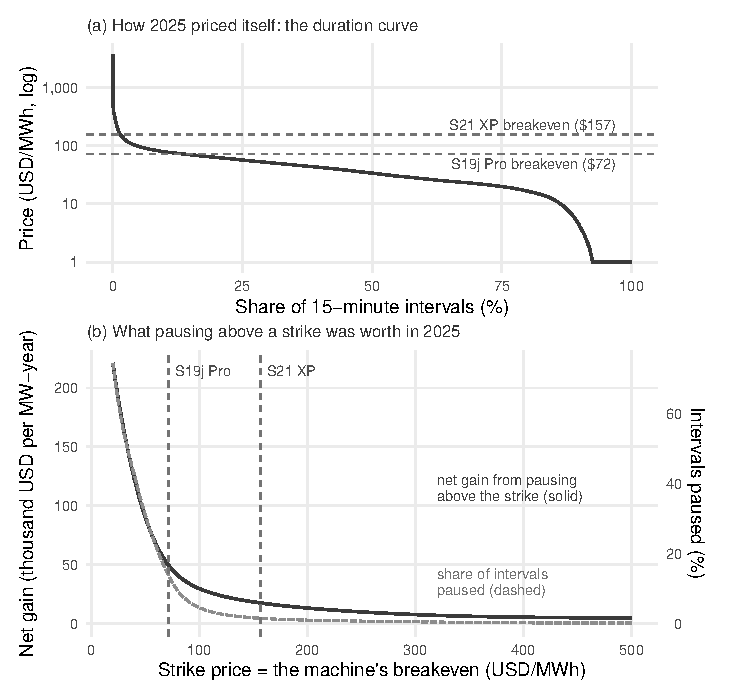
\includegraphics[width=\textwidth]{images/strike_sweep}
  \caption{
    What pausing was worth at LZ\_WEST in 2025, on 15-minute settlement prices. (a)~The price duration curve, with the Chapter~4 breakevens marked; prices below \$1 are drawn at \$1 on the log scale. (b)~The strike sweep: for a 1~MW always-on load that pauses whenever the price exceeds a strike, the annual net gain (solid, left axis) and the share of intervals paused (dashed, right axis), as a function of the strike. % fig-src: analysis/figures/fig_ch6_strike.R on analysis/data/ercot_rtm15_spp_loadzones_2021on.csv.gz (ERCOT MIS 13061)
  }
  \label{fig:strike-sweep}
\end{figure}

Panel~(b) prices the option directly. For every possible strike, it sums what a one-megawatt load would have saved by pausing whenever the price exceeded that strike, over the whole of 2025. Read off the two breakevens: pausing above \$72 earned the S19j~Pro fleet about \$49,000 per megawatt-year, for pausing about 14~percent of intervals, some 1,200 hours. % src: fig_ch6_strike.R console (S19j Pro strike $71.6: $49,116/MW-yr, 13.71%, 1201 h)
Those hours came as 1,018 separate pauses on 297 days: two in five lasted a single quarter-hour and three in five no more than 30 minutes, and the single quarter-hours earned about \$1,000 between them, 2~percent of the total. % src: analysis/checks/ch6_strike_events.R console (LZ_WEST 2025, strike $71.6, runs of consecutive intervals above it: 1,018, median 30 min, mean 1.18 h; 605 of two intervals or fewer = 59.4%; 408 of one interval = 40.1%, worth $1,032 = 2.1% of $49,116; 297 days with a run)
Pausing above \$157 earned the S21~XP fleet about \$17,000 per megawatt-year, for pausing 1.5~percent of intervals, about 130 hours. % src: fig_ch6_strike.R console (S21 XP strike $156.5: $17,280/MW-yr, 1.45%, 127 h)
For scale, running that megawatt around the clock at the index cost about \$370,000 in 2025; the S19j~Pro's option was worth an eighth of the entire power bill. % src: analysis/checks/ch6_contract_pnl.R (RT index $369,454/MW-yr; 49,116/369,454 = 13.3%)

Three readings. First, the money is concentrated: the sweep's steep left side says most of the value lives in the few hundred most expensive hours, which is why Chapter~5 spent so much engineering on catching spikes rather than on shaving averages. % src: ch6_strike_events.R console (the most expensive 200 hours hold 67.3% of the $49,116, the most expensive 400 hours 83.1%)
Nor is it reliably a summer story: in 2025 June to September earned 17~percent of the year, December and January together almost twice as much, and ten days from November to February about a third. On each year's own strike, the same four summer months had carried half the option in 2022 and four-fifths in 2023. % src: ch6_strike_events.R console, seasonality block (2025 at $71.6: Jun-Sep $8,516 = 17.3%; Dec + Jan $15,440 = 1.81 times; the ten best days of Jan, Feb, Nov and Dec $17,154 = 34.9% of the year; own-day strike through ch9_hashprice(), the moving strike of sell_vs_mine.R: Jun-Sep 51.0% of 2022's $131,251 and 79.3% of 2023's $237,653)
Second, the option is worth almost three times as much on the \emph{older} machine. That is Chapter~4's operating leverage arriving on the trading desk: the closer a machine lives to its breakeven, the more often the market crosses it, and the more its off switch earns. The marginal machine holds the fleet's most valuable option. % src: fig_ch6_strike.R console ($49,116 / $17,280 = 2.84)
Third, the sweep is a ceiling: it decides each interval on that interval's own settlement point price, which nobody can read until the interval is over. Decided one settlement interval late instead, with no forecast at all, the \$72 strike kept about \$44,000 in 2025, nine-tenths of the sum; Chapter~9 prices that executable version with each year's own strike. % src: ch6_strike_events.R console (pause when the previous interval's settlement point price exceeds $71.6, booked at each interval's own price, so a late pause into a cheap interval books a loss: $43,750 = 89.1% of $49,116, rows in chronological order through the repeated autumn hour; file order gives $43,749)
A site that must hold every pause and every restart for 30 minutes still keeps about \$42,000, in 869 pauses, and Chapter~5's loop cycles far less than either: it rides the moderate crossings at a lower power target and leaves the pause to a backstop that tripped 0.12 to 0.53 times a day in the backtests (Section~\ref{sec:threerules}). % src: ch6_strike_events.R console, lagged minimum-runtime block (30-minute minimum down and up: $42,358 in 869 pauses = 96.8% of the lagged $43,750); chapter 5 sec:threerules (analysis/ch5-backtest/output/trend_study/multizone_rtm15.csv stops_day: 0.12 to 0.53 pauses per day; LZ_WEST S19j Pro TEST-2025-26 0.53, 284 pauses)

The same settlement data also prices the rest of the contract menu, and Table~\ref{tab:contract-pnl} does so for a flat megawatt in 2025.

\begin{table}[h]
  \centering
  \footnotesize
  \setlength{\tabcolsep}{4pt}
  \begin{tabular}{lrrr}
    \hline
    \textbf{Contract shape} & \textbf{2025 average} & \textbf{Hours/yr} & \textbf{Flat 1 MW} \\
    \hline
    Real-time index (15-min) & \$42.18/MWh & 8,760 & \$369,454 \\
    Day-ahead index (hourly) & \$42.72/MWh & 8,760 & \$374,193 \\
    Fixed \$27.00 (Odessa PPA) & \$27.00/MWh & 8,760 & \$236,520 \\
    Fixed \$43.95 (Corsicana price) & \$43.95/MWh & 8,760 & \$385,002 \\
    \hline
    5x16 window, realized average & \$41.34/MWh & 4,080 & \\
    2x16 window, realized average & \$32.31/MWh & 1,760 & \\
    7x8 window, realized average & \$49.29/MWh & 2,920 & \\
    \hline
  \end{tabular}
  \caption{What a megawatt cost at LZ\_WEST in 2025, by contract shape. Block windows follow the ICE futures definitions \autocite{ice2026ercotnorthpeak,ice2026ercotnorth7x8}; their rows show the realized index average inside each window, a hindsight benchmark rather than a price anyone was quoted in advance. Fixed prices are the two disclosed in SEC filings, applied to every hour of the year; Riot's Corsicana block itself excludes July and August \autocite{cipher10k2024,riot10k2024}. The flexibility option of Section~\ref{sec:strikevalue} comes on top of, and is the same under, every row that permits pausing or sell-back.} % src: analysis/checks/ch6_contract_pnl.R console; fixed prices from cipher10k2024 and riot10k2024; window definitions from ice2026ercotnorthpeak and ice2026ercotnorth7x8
  \label{tab:contract-pnl}
\end{table}

The day-ahead index cost 1.3~percent more than the real-time index. That is what knowing each hour's price a day early happened to cost in 2025, measured after the year closed; nobody quotes it in advance, and it moves from year to year. At LZ\_WEST the day-ahead average ran 2.4, 8.8 and 3.4~percent above the real-time average from 2022 to 2024, and 2.1~percent below it in 2021, the year of Winter Storm Uri; without that February, 2021 would have come out 2.9~percent above as well. Arbitrage keeps the two annual averages within a few percent of each other, even while the two prices in a single hour still differ widely, as Chapter~3 measured. % src: ch6_contract_pnl.R console (LZ_WEST annual DAM minus RT means, MIS 13060 vs 13061: 2021 -2.13%, 2022 +2.37%, 2023 +8.84%, 2024 +3.38%, 2025 +1.28%; 2021 ex Feb +2.87%; 2025 flat 1 MW 374,193 vs 369,454); ch3 quantifies the ~$17 average absolute hourly DART gap
And the block rows are upside down. Everywhere in the textbook world, nights are cheap and weekday daytime is dear; at LZ\_WEST in 2025, the overnight 7x8 window averaged \$49 while the weekday-daytime 5x16 averaged \$41, and the cheapest power of the week was a weekend afternoon at \$32. % src: ch6_contract_pnl.R console (7x8 49.29; 5x16 41.34; 2x16 32.31)
The old off-peak discount did not shrink; it changed sign. Something structural did that, and it is the subject of Sections~\ref{sec:batteries} and~\ref{sec:duck}, because the same force is reshaping what every row of this table will look like next year.

\section{When the Miner Owns the Generator}
\label{sec:ownergen}

Riot and Cipher resell power they contracted for. The step beyond is to own the plant, and on the public record almost no miner in ERCOT has taken it with a plant that sells into the market. MARA bought a Texas wind farm in 2025, 114~MW of turbines with 240~MW of interconnection capacity in Hansford County, for \$49~million; but Hansford County sits in the upper Panhandle, and the federal generator inventory lists the county's one 114~MW wind plant in the Southwest Power Pool's balancing area, not ERCOT's \autocite{mara10k2025,eia860m2026}. % src: mara10k2025 (Note 3: Feb 14, 2025 acquisition, $49.2M, 114 MW nameplate, 240 MW interconnection); eia860m2026 Operating sheet (Plant ID 56905, Great Plains Windpark LLC, Hansford County TX, 114.0 MW onshore wind, Balancing Authority Code SWPP, operating since 2009); consistent with fig_ch3_lz_map.R's "upper Panhandle" gap
Soluna, the most visible behind-the-meter miner, describes its Texas sites as co-located with wind farms belonging to its power partners \autocite{soluna10k2025}. % src: soluna10k2025 (Dorothy "co-located with Briscoe Wind Farm"; Kati "powered entirely by the Las Majadas wind energy project"; Soluna works "with renewable energy developers and power partners")
Riot's 2025 annual report does not mention natural gas generation at all, and Cipher says only that it will evaluate behind-the-meter generation where appropriate \autocite{riot10k2025,cipher10k2025}. % src: riot10k2025; cipher10k2025 ("evaluate opportunities for behind-the-meter generation where appropriate")
ERCOT's rules for selling power also shape the sell-back contracts above.

To sell a megawatt-hour into ERCOT a mine must pass four gates. It registers with the commission before its first day of generation: as a power generation company if it means to sell, whatever its size, or as a self-generator if it means only to serve itself and its plant is a megawatt or more \autocite{puct25109}. % src: puct25109 (16 TAC 25.109(a)(1): PGC registration before the first day of generation, no MW floor; (a)(2): self-generator registration for facilities rated 1 MW or more that are not a PGC)
It enters ERCOT's generator interconnection process, which applies to any unit of a megawatt or more and to any Settlement Only Generator, of any size, a class the fourth gate explains. It pays an interconnection request fee of \$14,000 for a new generator of ten megawatts and up, \$8,000 below that or \$2,300 for a settlement-only unit on the distribution system, and a \$3,000 fee for the full interconnection study \autocite{ercotplanningguide2026,ercotfeeschedule2025}. % src: ercotplanningguide2026 sec. 5.2.1; ercotfeeschedule2025 (interconnection request fees $14,000 / $8,000 / $2,300 SODG; FIS application $3,000)
The fees are the cheap part of that gate. Under the commission's rule the wires utility pays for the transmission upgrades a plant at transmission voltage needs; the plant pays for its own step-up transformers and protection and, under agreements signed after 2025, for interconnection facilities beyond an allowance of \$14~million at 138~kV or less and \$20~million above, in 2024 dollars \autocite{puct25195}. % src: puct25195 (16 TAC 25.195, effective March 7, 2024, Project No. 55566, read 2026-09-27: (b)(1) transmission-level generator, interconnected at or above 60 kV; (f)(1) generator pays "step-up transformers and protective devices at the point of interconnection"; (f)(2), SGIA executed on or before December 31, 2025: TSP pays any new transmission facilities; (f)(3), SGIA executed after December 31, 2025: generator pays interconnection-facility costs above the allowance, TSP pays "any transmission system upgrades"; (f)(3)(A)(i) allowance from January 1, 2026 based on the 2024 amounts of $14,000,000 (138 kV or less) and $20,000,000 (above), adjusted each year by CPI under (A)(ii); (f)(3)(C) above-allowance costs directly billed, collectable as CIAC before construction; (e)(1) a deposit or other security may be required, returned under (e)(1)(A) once service begins)
It registers with ERCOT, for \$500, as a resource entity, the market's name for whoever owns or controls a generator, a battery or a load resource, and it must designate a Qualified Scheduling Entity, the intermediary Chapter~7 describes: a firm it hires or, once it qualifies as one, itself \autocite{ercotfeeschedule2025,ercot2026protocols}. % src: ercotfeeschedule2025 (Resource Entity registration $500); ercot2026protocols sec. 2 (Resource Entity: "An Entity that owns or controls a Generation Resource, an Energy Storage Resource (ESR), a Settlement Only Generator (SOG), or a Load Resource and is registered with ERCOT as a Resource Entity"), sec. 16.5.1.1(1) (each Resource Entity applicant "shall designate" a QSE), sec. 16.2.3.2(1) ("a Resource Entity serving as its own QSE"), sec. 16.2.1 (QSE qualification criteria)
The gate that matters is the fourth, the choice of class. A \glossaryterm{settlement-only-generator}{Settlement Only Generator} is paid for what it exports and nothing else: it may not offer energy, may not be committed or dispatched by ERCOT, and may not sell ancillary services \autocite{ercot2026protocols}. % src: ercot2026protocols sec. 2 (Settlement Only Generator definition)
A full generation resource may do all of those things and in exchange takes on continuous telemetry and a standing offer whenever it is online, the plumbing Chapter~7 describes, plus the duty to run when ERCOT commits it for reliability.

What the grid pays is the price at the generator's own node. A full resource and a Settlement Only Generator normally collect the time-weighted average of the five-minute prices at their bus over the settlement interval, with a floor of minus \$251 per megawatt-hour. The exception is the settlement-only class ERCOT keeps for Private Use Networks, the Settlement Only Transmission Self-Generator, a plant registered with the commission as a self-generator at the first gate. ERCOT settles such a network's net export at the load zone price, which spares it the gap between its node and the zone that West Texas plants live with, in a year when 91~percent of ERCOT's congestion cost arose inside zones rather than between them \autocite{ercot2026protocols,potomac2026somercot}. % src: ercot2026protocols secs. 6.6.1.1 (Resource Node price: time-weighted five-minute LMPs plus the reliability deployment adder, floored at -$251/MWh), 6.6.3.8(1)-(2) (SODG and SOTG paid at their bus, save units that opted out under (5), closed to units not operating or contracted by January 1, 2019, and, under (1)(b), sites where storage is more than half the SOG nameplate), sec. 2 (SOG "comprised of" SODG, SOTG and SOTSG; SOTSG: "connected to the ERCOT transmission system with a rating of one MW or more and is registered with the Public Utility Commission of Texas (PUCT) as a self-generator", registered with ERCOT and modeled under 3.10.7.3), 3.10.7.3(1)(c) ("Energy delivered to ERCOT from an SOTSG shall be settled in accordance with Section 6.6.3.2 ... at a Load Zone"), 6.6.3.2(1)(h) (SOTSG generation in the Load Zone imbalance); the word "self-generator" is kept for the commission's registration class of the first gate and for the name of the ERCOT class that requires it; potomac2026somercot p. 72 (91% intrazonal in 2025)
Generation pays no ERCOT fee on its output; the administration fee falls on metered load only \autocite{ercot2026protocols}. % src: ercot2026protocols sec. 9.16.1 (System Administration Fee on Adjusted Metered Load)
And the captured prices of Section~\ref{sec:btm}, \$19 for wind and \$21 for solar, are what ERCOT's wind and solar plants actually collected on average in 2025: less than half the zone price a load pays. % src: potomac2026somercot p. 20

An owner faces one choice every interval: burn the megawatt-hour into hashes, or sell it. Mining earns the machine's value of the energy, the strike of Section~\ref{sec:arbitrage}; selling earns the node price. For a plant that runs whatever the price, as a wind farm does, any fuel is spent either way and drops out of the choice; a gas plant has a third choice, to stay off, and its rule is a different one. So the owner mines while the price is below the strike and sells when it rises above, which is the same threshold as the buyer who pauses. A buyer pausing above the strike avoids a loss; an owner selling above the strike captures a gain; the sum of price over strike, taken over the hours when it is positive, is identical. For such a network, whose net export is settled at the zone price, the option to sell is therefore worth exactly what panel~(b) of Figure~\ref{fig:strike-sweep} said the option to pause was worth in hindsight: about \$49,000 per megawatt-year for an S19j~Pro fleet in 2025 and \$17,000 for an S21~XP fleet. A plant paid at its own node runs the same rule against that node's price; the captured prices above say how much lower that price runs on average, and whether the gap closes in the scarcity hours is a question about the plant's own bus that this book does not price. % src: fig_ch6_strike.R console ($49,116 and $17,280 per MW-yr); analysis/checks/sell_vs_mine.R (identity: sum of max(P - V, 0) is the same sum whether the MWh was avoided or sold)
The option looks small only because an owner measures it against the whole revenue of the machines, about \$630,000 per megawatt-year for the S19j~Pro, while a spot buyer measures the same dollars against a margin of about \$260,000, the machines' revenue less the power bill. % src: sell_vs_mine.R console, "2025 denominators" block: revenue $628,351 (mean moving strike $71.7 over all 8,760 h of 2025), power bill $369,454, margin $258,897

And it pays out like insurance. Run the same rule with each year's own hashprice, so that the strike moves as the machines' economics moved: the S19j~Pro's strike stood near \$440 in 2021 and the option still paid about \$960,000 per megawatt-year to a plant that kept running through the February storm, 94~percent of it in that one week; in 2023 it paid about \$240,000; in 2025 about \$51,000, a shade above the fixed-strike figure because the strike drifted with hashprice through the year \autocite{ercotrtmhist}. % src: analysis/checks/sell_vs_mine.R console, moving-strike table (2021 $957,665, of which Feb 14-20 $895,877 = 94%; 2023 $237,653; 2025 $51,499 per MW-yr; strikes $438 / $104 / $72); real-time settlement prices from ERCOT MIS report 13061
Once the gates are passed it costs nothing more to hold and pays little in a calm year; in 2021, a scarcity year, it paid, almost entirely in one week, about a quarter of what the machines earned all year, at a \$9,000 cap that today's rules no longer allow (Section~\ref{sec:ordc}). % src: sell_vs_mine.R console, "2021 denominators" block (sell option $957,665 against revenue at the moving strike, about 25%); the $9,000 cap of 2021: chapter 3 sec:ordc (ercot2021hcapnotice, HCAP $9,000 until January 1, 2022; potomac2021som p. vi, "the VOLL and HCAP of $9,000"); today's rules: chapter 3 sec:ordc (puct25509 (b)(6)(B) HCAP $5,000 and (c) the Emergency Pricing Program)
That week is also where the identity with the buyer breaks: a buyer who paused kept those dollars whatever happened upstream, while an owner kept them only on the megawatt-hours its plant delivered, in a week when about half of ERCOT's generation was offline \autocite{ERCOTUpdate2021}. % src: ch2 sec. on Uri (ERCOT Apr 27, 2021 update: 52,037 MW unavailable at the worst point, Feb 16)
The one place the owner does better than a plant that must sell is the roughly 490 hours of 2025 in which West Texas prices went negative: selling those hours cost money, and mining them did not. % src: sell_vs_mine.R console, "2025 denominators" block (count of negative-price 15-minute intervals in LZ_WEST / 4)

Few miners own generation because the prize of owning was never the electrons. At the captured prices above, a wind farm's energy is worth less to its owner than a mine would pay for it, so the generator would rather sell across the fence to a mine than into the grid, and the mine collects most of the discount by contract without buying a single turbine. The scarce thing is the plant's interconnection, in a market where requests in the large-load queue Chapter~3 described run to several times the system's peak, and a miner gets it by sitting behind the plant's meter, not by owning the plant. That is what the behind-the-meter arrangements of Section~\ref{sec:btm} are really buying.

\section{The Competition Arrived: Batteries}
\label{sec:batteries}

The strike sweep of Figure~\ref{fig:strike-sweep} pays out of price extremes: the option earns when prices spike, and to a lesser degree the bill shrinks when prices go negative. A miner holding that option should therefore watch, with professional interest, the one asset class whose entire business is deleting price extremes: grid batteries, which ERCOT calls \glossaryterm{energy-storage-resource}{energy storage resources} (ESRs). A battery buys the trough and sells the peak; every megawatt of it lifts the floor and shaves the spike that the miner's option was written on.

They arrived fast. Counting operating units by their in-service dates, ERCOT's battery fleet grew from about 4.4~GW of nameplate capacity at the start of 2024 to 8.5~GW a year later, 14.2~GW by the start of 2026, and 18.1~GW by mid-2026 \autocite{eia860m2026jul}. % src: fig_ch6_batteries.R console on analysis/data/ercot_capacity_additions_2026-07.csv (EIA-860M July 2026)
The market monitor's own ledger runs higher still, over 17~GW and 31,500~MWh by the end of 2025, up almost 80~percent in a year, with average duration stretching from 1.67 to 1.83 hours; the two counts differ in what they include and when, but they agree on the slope \autocite{potomac2026somercot}. % src: potomac2026somercot, pp. ii, 21-22 (IMM end-2025 >17 GW vs EIA-860M in-service 14.2 GW at 2026-01: different counting bases, both quoted as their own)
On a summer evening in 2025 the fleet was supplying an average of 4~GW in the eight-p.m.\ hour, filling the gap that solar leaves as it sets \autocite{eia2025ercotmix}. % src: eia2025ercotmix

\begin{figure}[htbp]
  \centering
  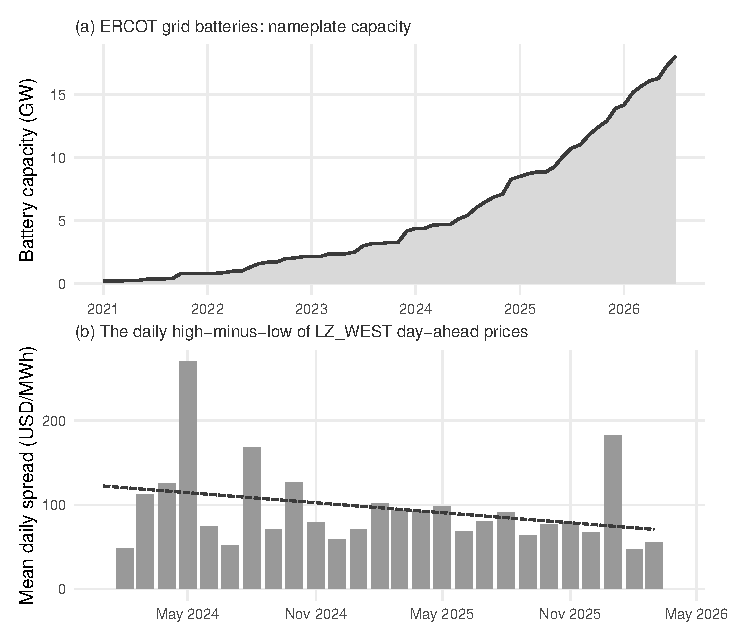
\includegraphics[width=\textwidth]{images/batteries_spreads}
  \caption{
    (a)~ERCOT grid batteries: cumulative nameplate capacity by operating date, from the federal generator inventory (EIA-860M, July 2026). (b)~The raw material of storage arbitrage: the monthly mean of each day's spread between the highest and lowest hourly day-ahead price at LZ\_WEST, with a linear trend. As the fleet roughly tripled, the average daily spread compressed from \$112 in 2024 to \$82 in 2025. % fig-src: analysis/figures/fig_ch6_batteries.R; console: spread 2024 $112.4, 2025 $82.0; capacity from analysis/data/ercot_capacity_additions_2026-07.csv
  }
  \label{fig:batteries-spreads}
\end{figure}

The price effects are no longer conjecture; the market monitor states them outright. Price spikes in summer 2025 were 40~percent less frequent than in summer 2024, because the added storage absorbed the system's ramps \autocite{potomac2026somercot}. % src: potomac2026somercot, p. iii
The ancillary service markets, where batteries found their first profits, saturated even faster: the average price of ECRS collapsed from about \$77 per megawatt per hour of standby in 2023 to under \$10 in 2024, a drop the market monitor puts down to new supply, batteries above all \autocite{potomac2024som}. % src: potomac2024som pp. ii, vi (ECRS $76.77 -> $9.62; "This drop was caused by an increase in supply, particularly from energy storage resources (ESRs)"), as chapter 7 prints it; until 2026-09-26 this line added an unlabelled "part correction" inference from potomac2026somercot, cut to match chapter 7 (PER-3 review round)
By 2025 batteries dominated ancillary supply so thoroughly that their own ancillary revenue fell by more than a third even as their fleet grew \autocite{potomac2026somercot}. % src: potomac2026somercot, p. 23 (AS revenue fell >37%)
Figure~\ref{fig:batteries-spreads}(b) shows the version of this squeeze that a miner feels: the average daily high-minus-low spread at LZ\_WEST, the raw material of storage arbitrage and strike alike, compressed by more than a quarter from 2024 to 2025. One year's correlation is not proof of cause, but the direction matches what the monitor attributes to storage, and the mechanism is not subtle.

So are batteries simply eating the miner's lunch? Partly: every dollar in Figure~\ref{fig:strike-sweep}(b) is smaller than it would have been in 2023's wilder market. But two structural differences keep the trades distinct. A battery is duration-limited: at 1.8 hours of storage it must choose which spike to sell into, so its arbitrage saturates against its own fleet, which is exactly what the ancillary collapse shows. % src: potomac2026somercot, pp. 21-22 (average ESR duration 1.83 h at end-2025, as chapter-6.tex:234)
It also pays for every round trip: it gives back about 85~percent of the energy it takes in, so it buys about 1.2 megawatt-hours for every one it sells, and each cycle wears its cells a little \autocite{potomac2026somercot,nlr2025atbbattery}. % src: potomac2026somercot, p. 21 (ESR fundamentals: a net load, losses occur throughout the cycle, NREL 2024 ATB round-trip efficiency 85%); 1 / 0.85 = 1.18 MWh bought per MWh sold; nlr2025atbbattery (2025 ATB: roundtrip efficiency 85%; about one cycle per day, and degradation is a function of the usage rate of the model; fixed O&M carries augmentation to hold rated capacity over a 15-year life)
A pausing miner has no state of charge and owes no energy back: it can stay off for an hour or a week if the price demands it, and when it is not pausing it is not idle capital waiting for volatility; it is mining. The battery needs the spread to justify existing. The miner's option is a bonus written on top of a business that pays for itself at \emph{average} prices, so when the spreads get thin, the battery feels it first.

\section{Renewables and the Shape of the Day}
\label{sec:duck}

The second structural force is the reason the spreads existed in the first place. Wind and solar together supplied 34.6~percent of ERCOT's energy in 2024 and 37.5~percent in 2025, with all of the growth coming from solar, whose share jumped from 10.4 to 13.9~percent \autocite{ercot2025factsheet,ercot2026factsheet}. % src: ercot2025factsheet (2024: wind 24.2 + solar 10.4); ercot2026factsheet (2025: wind 23.6 + solar 13.9); potomac2026somercot confirms 10.4 -> 13.9
Solar output grew 49~percent in 2025 alone, and summer midday solar production doubled between 2023 and 2025, from about 12 to about 24~GW at noon \autocite{potomac2026somercot,eia2025ercotmix}. % src: potomac2026somercot (solar +49%, 6% curtailed); eia2025ercotmix (12 -> 24 GW summer noon)
Wind and solar bid into the market at their marginal cost, which is approximately zero, and when they cover enough of demand they set the price at their level: the market monitor counts hundreds of hours per year with prices at or below zero \autocite{potomac2026somercot}. % src: potomac2026somercot (zero-marginal-cost growth; hundreds of hours at or below $0/MWh)

\begin{figure}[htbp]
  \centering
  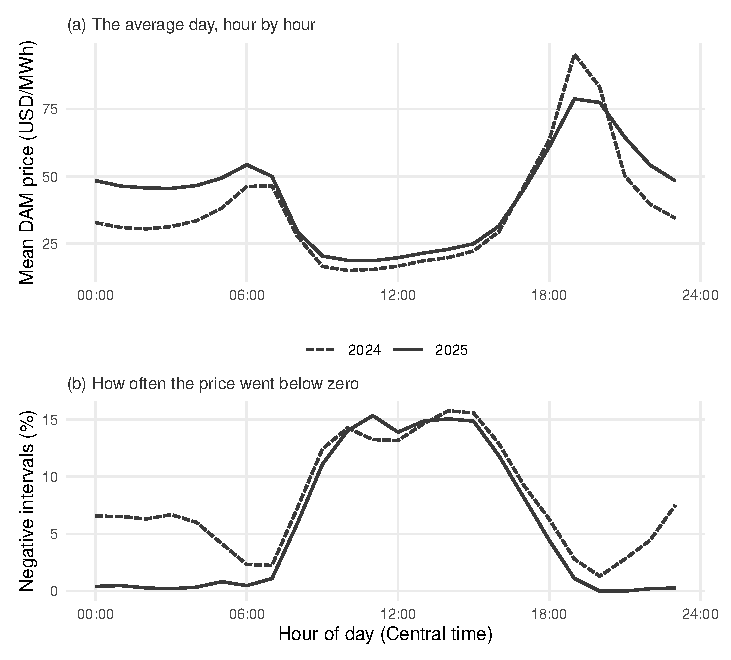
\includegraphics[width=\textwidth]{images/duck_lzwest}
  \caption{
    The duck at LZ\_WEST. (a)~Average day-ahead price by hour of day, by year: the midday trough deepens as solar grows, while the evening ramp holds its height. (b)~The share of 15-minute real-time settlement intervals with negative prices, by hour: overnight negatives, a wind signature, nearly vanished in 2025 as batteries and demand growth absorbed them; midday negatives, the solar signature, persist. % fig-src: analysis/figures/fig_ch6_duck.R; panel (a) on analysis/data/ercot_dam_spp_loadzones_2021on.csv.gz (ERCOT MIS 13060), panel (b) on analysis/data/ercot_rtm15_spp_loadzones_2021on.csv.gz (ERCOT MIS 13061)
  }
  \label{fig:duck}
\end{figure}

Plot the average price against the hour of the day and the result is the grid world's most famous silhouette, the \glossaryterm{duck-curve}{duck curve}: a deep belly at midday where solar floods the market and a steep neck in the evening when it withdraws. Figure~\ref{fig:duck} draws LZ\_WEST's duck. In 2025, midday hours averaged about \$21 while the evening ramp averaged about \$72: more than three times as much, a few hours apart on the same average day. % src: fig_ch6_duck.R console (2025: midday 11-15h DAM mean $20.8, evening 18-21h mean $72.4; the 2024 values are $17.7/$80.7)
Negative prices tell the same story with a twist: their overall share fell from 8.1~percent of intervals in 2024 to 5.6~percent in 2025, but the composition flipped, with the old overnight wind-driven negatives nearly disappearing while the midday solar negatives held on. % src: fig_ch6_duck.R console (negative share 8.1% 2024 -> 5.6% 2025; overnight negatives collapse)
Batteries charging through the cheap hours absorbed the negatives that fit inside their duration; the midday solar surplus still outruns them. The market monitor adds the system-level confirmation: the tightest hours of the ERCOT day have migrated from the traditional four-to-five-p.m.\ demand peak to the seven-to-nine-p.m.\ \glossaryterm{net-load}{net-load} peak, the hour when demand minus renewables is highest, which is the hour solar leaves \autocite{potomac2026somercot}. % src: potomac2026somercot (tightest period shifted from 4-5 p.m. to 7-9 p.m.)

This is what inverted Table~\ref{tab:contract-pnl}'s block rows. The 5x16 weekday-daytime window now contains the solar belly, so its average sags; the 7x8 night window contains no solar at all, so it holds firm; the weekend 2x16 combines the belly with weekend demand and becomes the cheapest shape on the menu. West Texas sharpens everything: the market monitor notes that the West zone managed to post both the highest average price of any zone in 2025 \emph{and} the most negative-price intervals, because the wind-and-solar-rich Panhandle is export-constrained while the demand-heavy Permian is import-constrained \autocite{potomac2026somercot}. % src: potomac2026somercot (West zone: highest average price, most negative intervals, most price spikes)
A flat consumer would call that the worst of both worlds. For a load that follows price, that is the best of both: deeper discounts to mine through and taller spikes to sell absence into, which is why it is this book's home zone.

For the miner, then, the renewable buildout helps on both sides of the ledger. It drags the \emph{average} down, which fattens the mining margin at any hashprice; and it steepens the \emph{shape}, which raises what flexibility earns. The daily price pattern rewards consumption at midday and curtailment during the evening ramp. Machines that pause in seconds suit that daily rhythm, plus the handful of days a year, winter ones included, when the price becomes a crisis. % src: ch6_strike_events.R console (2025: ten days of January, February, November and December hold 34.9% of the S19j Pro's option at $71.6)

\section{The Market Just Changed: RTC+B}
\label{sec:rtcb-firstlook}

Everything measured so far in this chapter was priced under market rules that ended in December 2025. On December~5, ERCOT switched on Real-Time Co-optimization plus Batteries (RTC+B), which it calls the most substantial change to the real-time market since the nodal design launched in 2010 \autocite{ercot2025rtcblive}. % src: ercot2025rtcblive (go-live Dec 5, 2025; "most substantial enhancement... since its inception in 2010")
The change is easy to state in this book's vocabulary: before, ERCOT bought energy every five minutes but reserved ancillary capacity a day ahead; now the real-time engine buys energy \emph{and} every ancillary product together, every five minutes, with battery state of charge modeled explicitly, so a megawatt can flow to whichever use is worth most right now. % src: ercot2025rtcblive (co-optimized energy + AS procurement in real time; battery SOC modeling)
The project was ordered by the Texas commission in 2019, took six years to build, and ERCOT projects the efficiency gain at over a billion dollars of wholesale cost per year \autocite{ercot2025rtcblive}. % src: ercot2025rtcblive (PUCT Project No. 48540, 2019 directive; Collins quote: "projected wholesale market savings exceeding one billion dollars annually")

The early reviews were undramatic, which for a market redesign is praise. Day-ahead ancillary prices spiked on the go-live day itself, then normalized within days; the market monitor put 15 of December's 24 priciest day-ahead Non-Spin hours on December 5 and attributed them to uncertainty about the change. The real-time market then worked as expected, with no major malfunction but a short stabilization list, until Winter Storm Fern gave it a real test in late January. Batteries repriced their day-ahead ancillary offers upward in every product, and the reason is structural: the redesign lets a resource sell reserves straight into real time, which makes a day-ahead position riskier for anything duration-limited \autocite{potomac2026somercot,ercotcmu2026feb}. % src: potomac2026somercot p. 40 (15 of 24 highest-priced December DAM Non-Spin hours on Dec 5, 2025; "AS prices normalized again a few days after RTC go-live"), Appendix I pp. A-2 to A-5 ("operating largely as expected without major dysfunctions"; Figure A2, ESR day-ahead AS offers repriced upward in all five products; p. A-3 gives the duration-constraint and sell-into-real-time reason and says the monitor predicted it); ercotcmu2026feb slides 1-2 and the RTC+B Stabilization Activities slide

\begin{figure}[p]
  \centering
  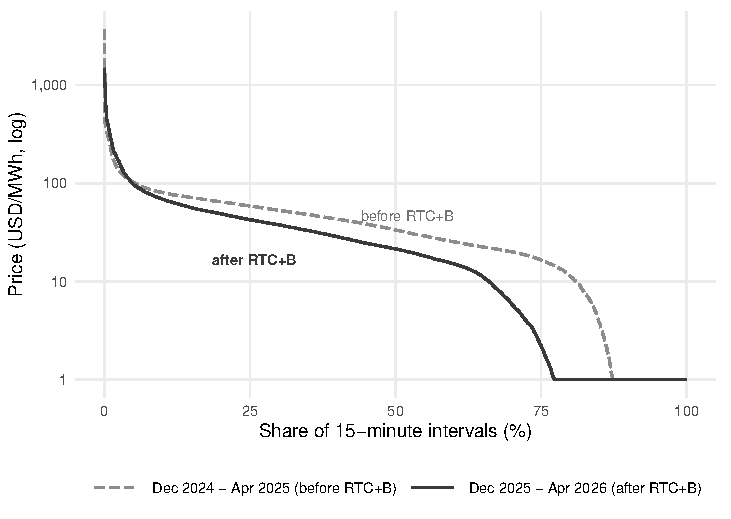
\includegraphics[width=\textwidth]{images/rtcb_volatility}
  \caption{
    A season-matched first look at prices under RTC+B: LZ\_WEST 15-minute settlement prices for December~5 to April~20, the winter before go-live against the first winter after. Duration curves on a log scale; prices below \$1 are drawn at \$1. The average fell, negative-price intervals doubled, the moderate tail thickened, and the extreme tail shortened. % fig-src: analysis/figures/fig_ch6_rtcb.R on analysis/data/ercot_rtm15_spp_loadzones_2021on.csv.gz (ERCOT MIS 13061)
  }
  \label{fig:rtcb}
\end{figure}

Figure~\ref{fig:rtcb} makes the comparison this book can make honestly: the same calendar window, December~5 through April~20, in the last winter of the old rules and the first winter of the new ones, at LZ\_WEST on settlement prices. The average fell from about \$42 to \$34/MWh. % src: fig_ch6_rtcb.R console (season-matched mean $42.56 -> $33.60)
Negative-price intervals doubled, from 9.5 to 18.8~percent of the window. % src: fig_ch6_rtcb.R console (negative share 9.54% -> 18.76%)
The extreme tail shortened, with the window's maximum falling from about \$3,700 to \$1,500, while the moderate tail thickened: the 99th-percentile price rose from about \$230 to \$300. % src: fig_ch6_rtcb.R console (max $3,686.94 -> $1,485; P99 $228 -> $295)

Every caveat belongs in the same breath as the numbers. This is one winter against one winter; each window contains one winter storm (Winter Storm Kingston before, Fern after); the battery fleet grew almost 80~percent and solar kept building through the comparison, so this figure measures RTC+B \emph{plus} everything else that changed; and the market monitor's first full assessment will not arrive until its next annual report \autocite{potomac2026somercot}. % src: potomac2026somercot (ESR +80% in 2025); fig_ch6_rtcb.R window definition (Kingston Feb 2025 in the before-window, Fern Jan 2026 after); labeled first look, not attribution
Call it a first look. But notice what each shift in it means for a flexible load: a cheaper average megawatt-hour, twice as many intervals that pay you to consume, and more frequent moderate spikes for the strike to harvest. Against that, it has fewer of the catastrophic prices in which, as Section~\ref{sec:strikevalue} showed, most of the option's value has lived. If the pattern holds, the new market pays flexibility more often and in smaller amounts, and a machine that earns its option in small bites, over and over, is built for that world.

\bigskip

The chapter's ledger, then. The contract sets your average cost and decides whether your off switch is connected to the market; the machine sets the strike; and in 2025 at LZ\_WEST the strike was worth about \$49,000 per megawatt-year on the marginal fleet in hindsight and \$44,000 decided one interval late, about an eighth of the power bill, before a single new market product enters the picture. % src: fig_ch6_strike.R console ($49,116); ch6_strike_events.R console (lagged $43,750); ch6_contract_pnl.R (RT index $369,454/MW-yr: 13.3% and 11.8%)
Batteries, renewables, and RTC+B are reshaping the prices underneath it, compressing the old spreads while multiplying the small ones. But pausing against price is still only the first way ERCOT pays a flexible load, and it is the passive one: the market never knows the miner is there; it just sees demand vanish above a threshold. The second way is louder. ERCOT runs standing markets that pay loads simply to be \emph{ready} to vanish on command, whether or not the command ever comes, and RTC+B just rebuilt those markets from the ground up. These are the ancillary service markets of Chapter~7.
